
\begin{enumerate}


\item A solid sphere is cut into two hemispheres. The ratio of the surface areas of the sphere to that of the two hemispheres taken together is:
	\begin{enumerate}    
\item $1:1$
    \item $1:4$
    \item $2:3$
    \item $3:2$
	\end{enumerate}

\item The volume of the largest right circular cone that can be carved out from a solid cube of edge $2 \, \text{cm}$ is:
	\begin{enumerate}    
\item $\frac{4\pi}{3} \, \mathrm{cu cm}$
    \item $\frac{5\pi}{3} \, \mathrm{cu cm}$
    \item $\frac{8\pi}{3} \, \mathrm{cu cm}$
    \item $\frac{2\pi}{3} \, \mathrm{cu cm}$
	\end{enumerate}

\item \textbf{Assertion (A):} The tangents drawn at the end points of a diameter of a circle are parallel.

\textbf{Reason (R):} The diameter of a circle is the longest chord.
\begin{enumerate}
    \item Both Assertion (A) and Reason (R) are true, and Reason (R) is the correct explanation of Assertion (A).
    \item Both Assertion (A) and Reason (R) are true, but Reason (R) is not the correct explanation for Assertion (A).
    \item Assertion (A) is true, but Reason (R) is false.
    \item Assertion (A) is false, but Reason (R) is true.
\end{enumerate}

\item $AD$ is a median of $\triangle ABC$ with vertices $A(5, -6)$, $B(6, 4)$, and $C(0, 0)$. The length of $AD$ is equal to:
	\begin{enumerate}    
\item $\sqrt{68}$ units
    \item $2\sqrt{15}$ units
    \item $\sqrt{101}$ units
    \item $10$ units
	\end{enumerate}

 \item If the distance between the points $\brak{3, -5}$ and $\brak{x, -5}$ is 15 units, then the values of $x$ are:
    \begin{enumerate}
    \item $12, -18$
    \item $-12, 18$
    \item $18, 5$
    \item $-9, -12$
    \end{enumerate}

    \item The center of a circle is at $\brak{2, 0}$. If one end of a diameter is at $\brak{6, 0}$, then the other end is at:
	\begin{enumerate}    
		\item $\brak{0, 0}$
		\item $\brak{4, 0}$
		\item $\brak{-2, 0}$
		\item $\brak{-6, 0}$
	\end{enumerate}

 \item In  the given figure, $ABCD$ is a qadrilateral.diagonal $BD$ bisects $\angle B$ and $\angle D$ both.
\begin{figure}[!ht]                                                                                         \centering
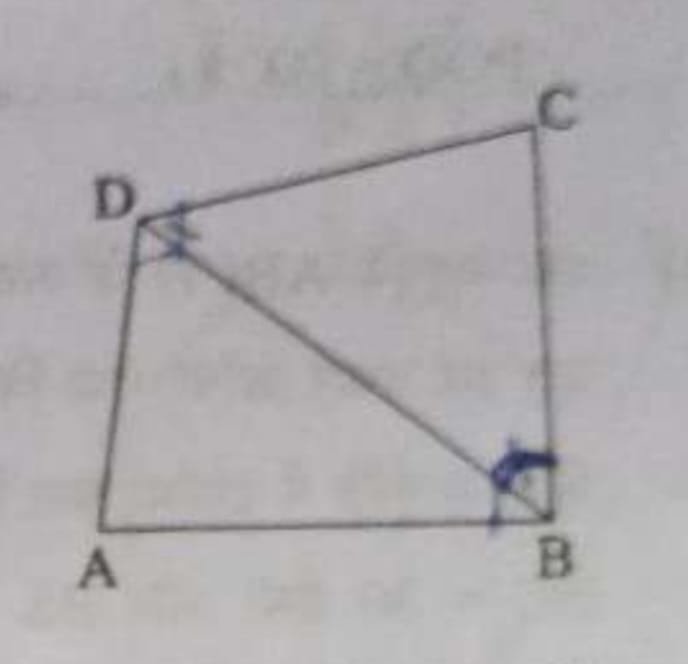
\includegraphics[width=\columnwidth]{figs/g1.jpg}
\label{fig:image 1}
\caption{image 1}                                                                                           \end{figure}\\
\text Prove that :                                                                                          \begin{enumerate}                                                                                           \item$\triangle ABD \sim \triangle CBD $\
\item $AB = BC$                                                                                             \end{enumerate}
\item Find the ratio in which the point $\brak{8, y}$ divides the line segment joining the points $\brak{1, 2}$ and $\brak{2, 3}$.. Also, find the value of  $y$.
\item $ABCD$ is a rectangle formed by the points $ A\brak{-1,-1}, B\brak{-1, 6}, C\brak{3, 6}$ and $D\brak{3
, 1}, P, Q, R$ and $S$ are mid-points of sides $AB, BC, CD$ and $DA$ respectively.Show that diagonals of the
 quadrilateral $PQRS$ bisect each other.
\item In the given figure,$AB$ is a diameter of the circle $O. AQ, BP$ and $PQ$ are tangents to the circle.p
rove that $\angle POQ = 90\degree$.
\begin{figure}[!ht]
\centering
	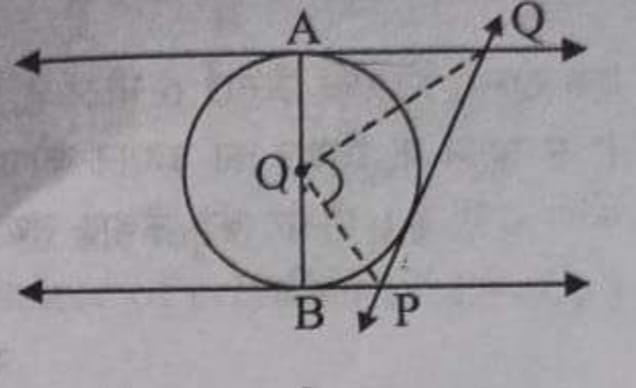
\includegraphics[width=\columnwidth]{figs/g2.jpg}
\label{fig:Image 2}
\caption{image 2}
\end{figure}
\item  A circle with centre $O$ and radius $8\mathrm{cm}$ is inscribed in a quadrilateral $ABCD$ in which $P
, Q, R, S$ are the points of contact as shown. If $AD$ is perpendicular to $DC, BC = 30\mathrm{cm}$ and $BS
= 24\mathrm{cm}$, then find the length $DC$.
\begin{figure}[!ht]
\centering
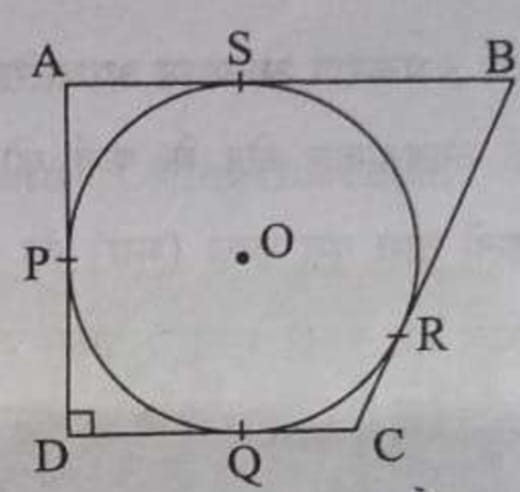
\includegraphics[width=\columnwidth]{figs/g3.jpg} 
\label{fig:Image 3}
\caption{image 3}
\end{figure}                                                                                                
\item The difference between the outer and inner radii of a hollow right circular cylinder of length $14\mathrm{cm}$ is $1\mathrm{cm}$. If the volume of the metal used in making the cylinder is $176\mathrm{cm}^3$, find the outer and inner radii of the cylinder.  
\item An arc of a circle of radius $21\mathrm{cm}$ subtends an angle of $60\degree$ at the centre. Find:
\begin{enumerate}                                                                                       
\item the length of the arc.
\item the area of the minor segment of the circle made by the corresponding chord.
\end{enumerate}  
\item If a line is drawn parallel to one side of a triangle to intersect the other two sides in distinct points, then prove that the other two sides are divided in the same ratio. 
\item In the given figure $PA,QB$ and $RC$ are each perpenicular to $AC$. if $AP = x,bq=y$ and $cr =z$,then
prove that $\frac{1}{x} + \frac{1}{z} = \frac{1}{y}$ 
\newpage
\begin{figure}[!ht]
\centering
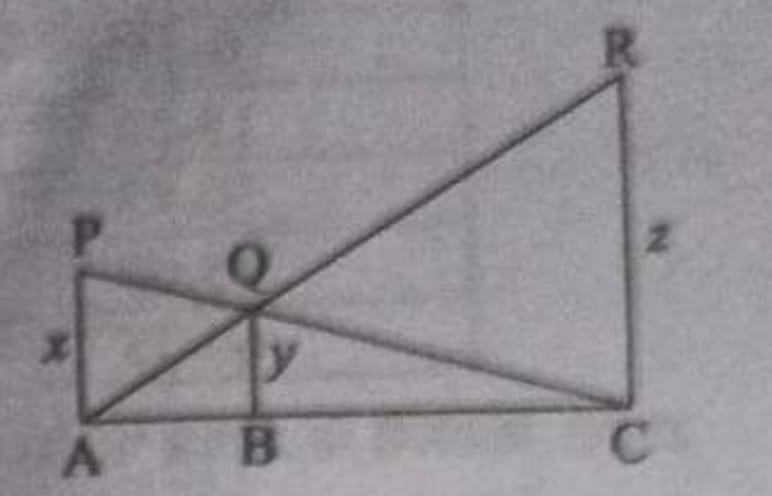
\includegraphics[width=\columnwidth]{figs/g4.jpg}   
\label{fig:image 4}
\caption{image 4}
\end{figure}
\item A backyard is in the shape of a triangle $ABC$ with right angle at $B AB = 7 m$ and $BC = 15 m$. A cir
cular pit was dug inside it such that it touches the walls $AC. BC$ and $AB$ at $P, Q$ and $R$ respectively such that $AP=xm$.
\begin{figure}[!ht]
\centering
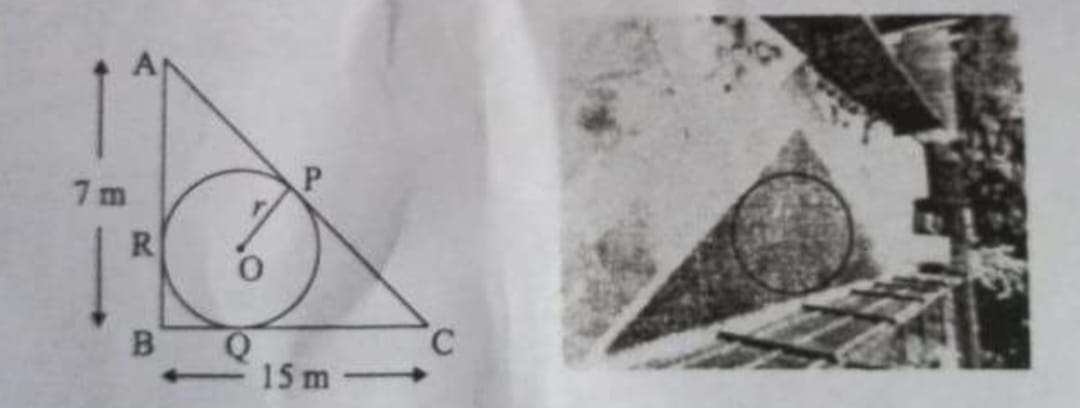
\includegraphics[width=\columnwidth]{figs/g5.jpg}
\label{fig:image 7}
\caption{image 7}
\end{figure}
\text Based on the above information,answer the following question:\
\begin{enumerate}  
\item find the length of AR in terms of $x$.\ 
\item write the type of quardrilateral of $BQOR$.\ 
\item Find the length C in terms of x and hence find the value of $x$.\
\item Find $x$ and hence find the radius r of circle.
\end{enumerate}

\end{enumerate}
